\section{Resultados}

\subsection{Red de interacciones y robustez}

En la imagen Figure~\ref{stringhits} se muestra la red de interacciones del ser humano con las proteínas del SARS-CoV. Como podemos ver el SARS-CoV interacciona con 89 proteínas humanas, produciendo un total de 475 interacciones. 

\begin{figure}[h]
	\centering
		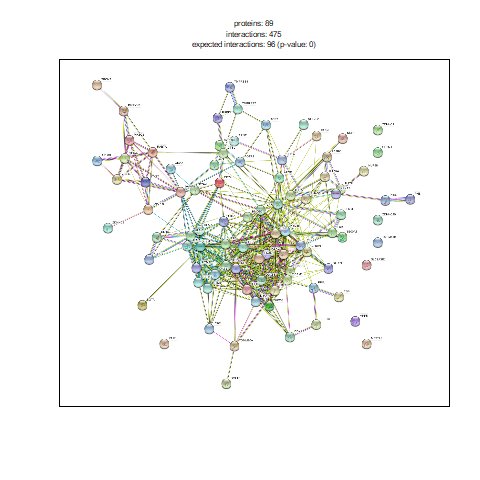
\includegraphics[width=70mm,scale=1.2]{figures/string_hits.png}
		\caption{\textit{Red de interacciones del SARS-CoV con las proteínas humanas}}
		\label{stringhits}
\end{figure}

Tras eliminar los nodos que no están conectados, hemos obtenido la red real de interacciones que podemos ver a continuación. Sin embargo hay demasiadas conexiones como para poder distinguir los nodos. Es por ello que realizaremos los pasos siguientes de clustering, para así poder extraer la información relevante de la red. Podemos observar la red de interacciones en la figura Figure~\ref{hitsnetwork}.

\begin{figure}[h]
	\centering
		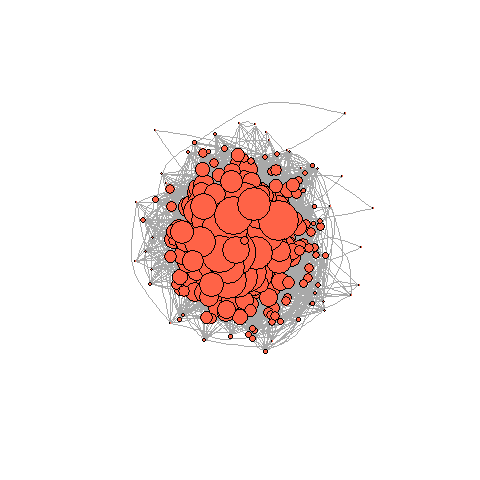
\includegraphics[width=70mm,scale=1.2]{figures/hits.network_graph.png}
		\caption{\textit{Red de interacciones del SARS-CoV con las proteínas humanas tras un proceso de filtrado}}
		\label{hitsnetwork}
\end{figure}


Antes de empezar con ese proceso vamos a estudiar diferentes aspectos de nuestra red. En primer lugar si observamos la imagen Figure~\ref{degree}, vemos que el la distribución de grado sigue la ley de potencias, por lo tanto nuestra red sigue un modelo de free-scale, lo cual era predecible al estar tratando con una red real. 

Podemos  ver una gran cantidad de hubs.

\begin{figure}[h]
	\centering
		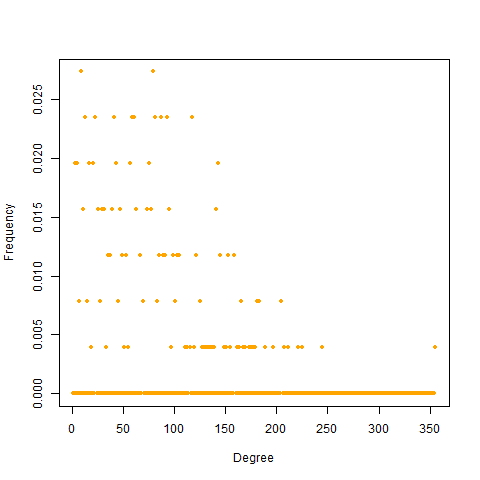
\includegraphics[width=70mm,scale=1.2]{figures/degree_distribution.png}
		\caption{\textit{Distribución de grado}}
	    \label{degree}
\end{figure}

El coeficiente medio de agrupamiento es de 0.605, lo cual es bastante alto. Además se puede observar la característica propia de las redes reales la cual afirma que conforme el grado de los nodos aumenta, el coeficiente de agrupamiento disminuye. La gráfica del coeficiente de agrupamiento esta en la Figure~\ref{coefclust}.

\begin{figure}[h]
	\centering
		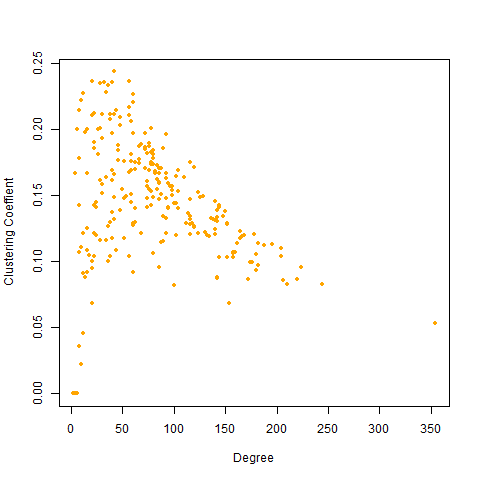
\includegraphics[width=70mm,scale=1.2]{figures/coeficiente_agrupamiento.png}
		\caption{\textit{Coeficiente de Agrupamiento}}
		\label{coefclust}
\end{figure}

La distancia media entre nodos es de 2.03, una medida muy pequeña que puede significar que los nodos tienen un alto índice de conexiones. Esta medida es la que le da la propiedad de mundo pequeño, es decir, la distancia entre nodos elegidos al azar en una red es muy pequeña. Esto se puede observar de forma visual en la Figure~\ref{distance}.

\begin{figure}[h]
	\centering
		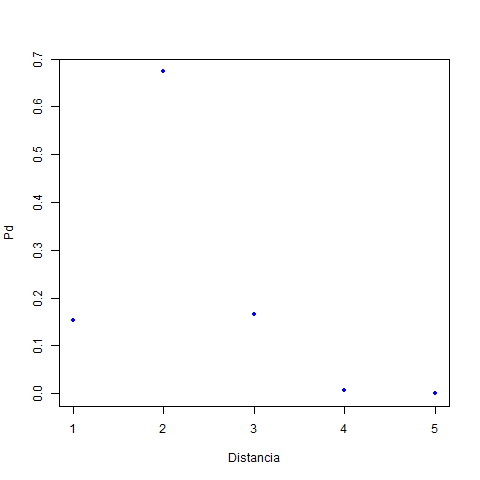
\includegraphics[width=70mm,scale=1.2]{figures/distancia.png}
		\caption{\textit{Distancia entre nodos}}
		\label{distance}	
\end{figure}

Por último vamos a estudiar la robustez de nuestra red. Para poder estudiar cual es la capacidad de nuestra red de mantener sus funciones frente a la presencia de "ataques" y ver cuán de adaptable es, usamos la robustez. Podemos observar en la Figure~\ref{ataques} que para ataques aleatorios es bastante robusta, mientras que para ataques dirigidos es más débil. Pues a que tenemos una red real, estos resultados resultan obvios, ya que es más fácil destruir una red si atacas a puntos estratégicos como son los hubs, dónde el tamaño de la componente conexa se reduce drásticamente cuando eliminamos una pequeña fracción de los nodos (hubs). 

\begin{figure}[h]
	\centering
	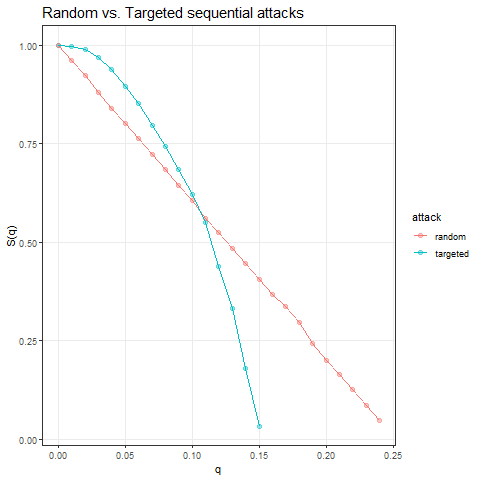
\includegraphics[width=70mm,scale=1.2]{figures/sequential_attacks.png}
	\caption{\textit{Robustez frente a ataques dirigidos y aleatorios}}
	\label{ataques}
\end{figure}

\subsection{Linked Communities}
En esta sección se explicarán los resultados obtenidos aplicar los métodos de comunidades enlazadas a nuestra red, para los cuales hemos usado el paquete linkcomm. Primero de todo, mencionar que las comunidades de una red son subredes que están altamente relacionados entre sí debido a que sus proteínas poseen algunas características similares. Estas pueden ser funciones biológicas, coeficiente de clustering, o tienen perturbaciones en su secuencia genética que pueden ser enlazadas a una enfermedad común.

Para la identificación de las comunidades más relevantes en nuestra red, hemos aplicado una función predefinida que devuelve el conjunto de las comunidades identificadas mediante la aplicación de un algoritmo de 'single clustering'. Se ha guardado una imagen Figure~\ref{comunidades} del resumen de estas comunidades para un resultado más visual.

\begin{figure}[h]
	\centering
	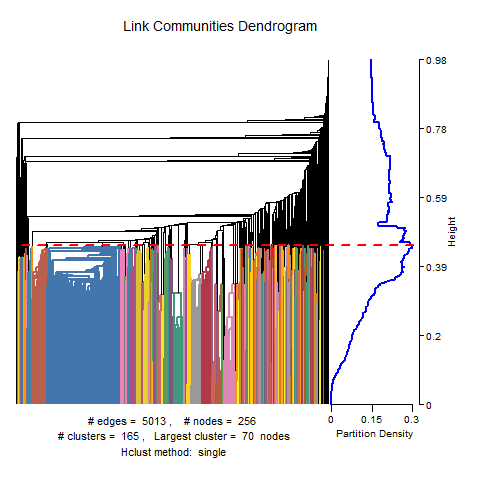
\includegraphics[width=70mm,scale=1.2]{figures/covid_lc_summary.png}
	\caption{\textit{Esquema de las comunidades obtenidas}}
	\label{comunidades}
\end{figure}

Podemos observar que este método ha definido 165 comunidades diferentes, la mayor de estas tiene 70 nodos lo cual podemos deducir que hay varias comunidades que comparten nodos en nuestra red.

Para poder analizar las comunidades y obtener las que consideremos más relevantes, han sido filtradas por tamaño y modularidad. Lo cual nos ha facilitado la búsqueda de la comunidad más grande y dos comunidades que tienen mayor modularidad ( y  respectivamente). Las gráficas generadas para este propósito son Figure~\ref{comTamaño} y Figure~\ref{comModularidad}.

\begin{figure}h]
	\centering
	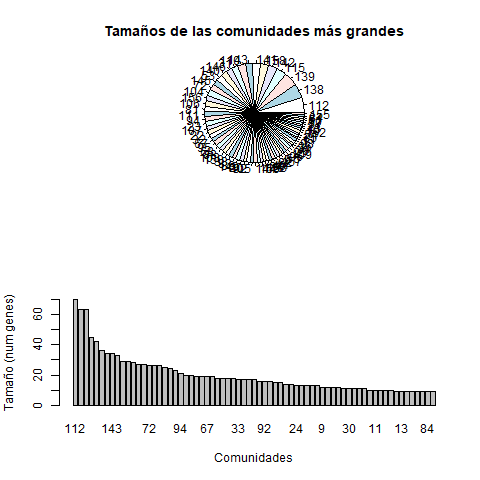
\includegraphics[width=70mm,scale=1.2]{figures/lc_larger_clusters.png}
	\caption{\textit{Comunidades por tamaño}}
	\label{comTamaño}
\end{figure}

\begin{figure}[h]
	\centering
	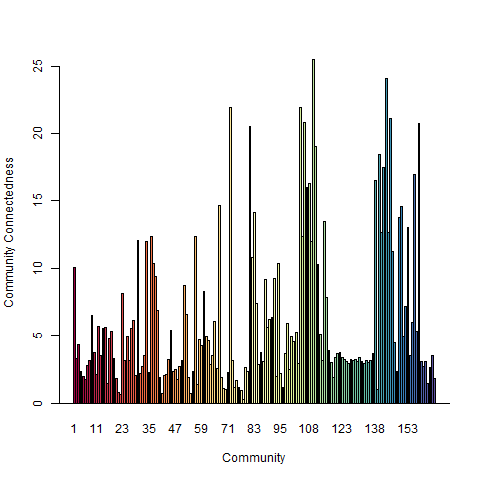
\includegraphics[width=70mm,scale=1.2]{figures/clusters_modularity.png}
	\caption{\textit{Comunidades por modularidad}}
	\label{comModularidad}
\end{figure}

Hemos podido extraer la comunidad 112 siendo esta la más grande y las comunidades 78 y 22 con una mayor modularidad. A estas comunidades encontradas se les realizará un enriquecimiento funcional para observar las funciones y características comunes que poseen y así poder sacar conclusiones adecuadas.

Para una mejor visualización de los resultados, se ha cambiado el diseño de la gráfica al de Fruchterman Reingold (se puede observar en la Figure~\ref{FRg}), mostrando solo nodos que pertenezcan a 10 o más comunidades.

\begin{figure}[h]
	\centering
	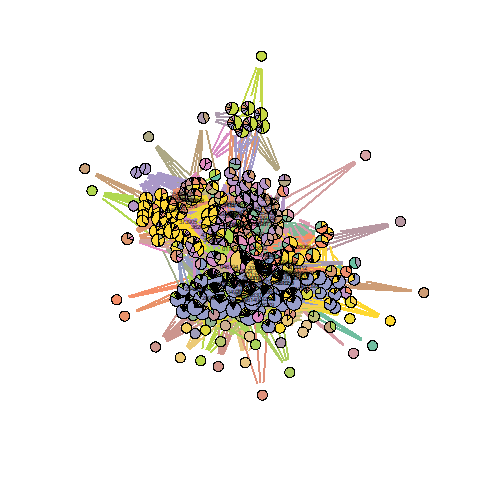
\includegraphics[width=70mm,scale=1.2]{figures/hits.network_layout_fruchterman.reingold_shownodesin_10.png}
	\caption{\textit{Fruchterman Reingold graph}}
	\label{FRg}
\end{figure}

Por otra parte, se han obtenido las comunidades anidadas y se han filtrado para que se muestren las que son independientes de las demás. Estas se observar en la Figure~\ref{anidadas}.

\begin{figure}[h]
	\centering
	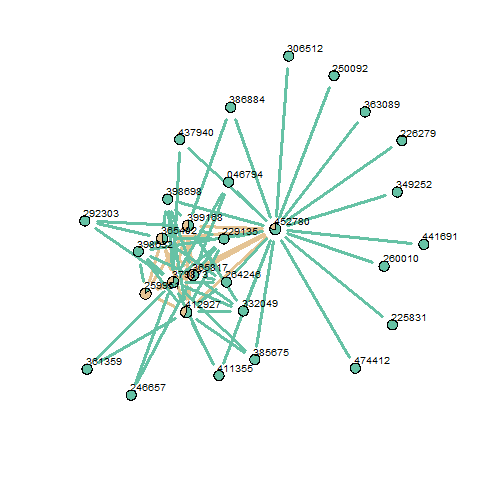
\includegraphics[width=70mm,scale=1.2]{figures/nested_comm.png}
	\caption{\textit{Comunidades anidadas}}
	\label{anidadas}
\end{figure}

\subsection{Enriquecimiento funcional}

En esta sección se van a mostrar los resultados obtenidos al realizar el enriquecimiento funcional con GO y con KEGG, mediante el uso de STRINGdb, para los clústeres elegidos.
Se ha guardado la información del enriquecimiento en archivos de tipo csv, y se va a mostrar una imagen de los mismos.

\subsubsection{Clúster 112}

\paragraph{Enriquecimiento con GO}

Entre las funciones biológicas obtenidas con el enriquecimiento con GO, se puede observar que algunas de ellas están relacionadas con la defensa del organismo, por lo que se puede deducir que son proteínas que forman parte del sistema inmunológico de nuestro organismo. Otras tantas funciones biológicas están asociadas con la regulación de diversos procesos biológicos.

\paragraph{Enriquecimiento con KEGG}

Las funciones biológicas en el enriquecimiento con KEGG están relacionadas con enfermedades/infecciones (malaria, hepatitis B, tuberculosis) por lo que se podríamos deducir que dichas proteínas forman parte de la respuesta inmunitaria del organismo ante dichas enfermedades o que las provocan.
Además de esto, se observan funciones biológicas relacionadas con vías biológicas del organismo, como son la vía de señalización de quimioquinas, la de detección de ADN citosólico...

\subsubsection{Clúster 78}

\paragraph{Enriquecimiento con GO}

GO no ha encontrado funciones biológicas asociadas al clúster elegido.

\paragraph{Enriquecimiento con KEGG}

En este caso, KEGG ha encontrado dos funciones biológicas asociadas al clúster: cáncer de tiroides y vías en el cáncer. Es por tanto que deducimos que las proteínas que forman parte de este clúster se ocupan de las vías principales del cáncer de tiroides, ya sea para detectarlo o provocarlo. 

\subsubsection{Clúster 22}

\paragraph{Enriquecimiento con GO}

En este caso se puede observar que las principales funciones biológicas de las proteínas pertenecientes a este clúster son de regulación, transporte y recepción, por lo que desempeñan funciones muy importantes en las rutas metabólicas del organismo. 

\paragraph{Enriquecimiento con KEGG}

Las funciones biológicas obtenidas por KEGG son más concretas: reabsorción de calcio regulada por factores endocrinos, ciclo de vesículas sinápticas, endocitosis, lisosoma, enfermedad de Huntington, invasión bacteriana de las células epiteliales y vía de señalización de la fosfolipasa D. Esta última está relacionada con la traducción de señales. Otras están relacionadas con enfermedades y sus causas.